% !TeX program = xelatex
% !TeX encoding = UTF-8
\documentclass[a4paper, 11pt, answers]{exam}

\usepackage[brazil]{babel}
\let\latinencoding\relax
\usepackage[T1]{fontenc}

\usepackage[no-math]{fontspec}
\usepackage{newpxtext, newpxmath}
\usepackage[a4paper, margin=2cm]{geometry}

\usepackage{siunitx}
\usepackage{fancyvrb}
\usepackage{graphicx}
\usepackage{caption}
\usepackage{siunitx}
\PassOptionsToPackage{hyphens}{url}
\usepackage[colorlinks,breaklinks=true,urlcolor=blue,linkcolor=black]{hyperref}
\def\UrlBreaks{\do\/\do-}
%\usepackage[hyphenbreaks]{breakurl}

\input{definition.tex}

\title{\titulo}
\author{\nomeAutorUm e \nomeAutorDois}
\date{\today}

\footer{}{}{\thepage}

\sisetup{
  binary-units = true
}

\renewcommand{\solutiontitle}{}

\fvset{
  gobble=4,
  frame = single
}

\graphicspath{{img/}}

\newcommand{\printtitle}{
  \begin{center}
    {\Large \scshape \titulo}\\[1em]
    {\nomeAutorUm, \raAutorUm}\\
    {\nomeAutorDois, \raAutorDois}\\[1em]
    Professor: Dr\@. \nomeProfessor, \centroProfessor\\
    {\itshape \campusFaculdade}
  \end{center}
}

\begin{document}
  \printtitle

  \begin{questions}
    \section*{Parte 01}
    \question
Interação básica HTTP.

\begin{parts}
  \part
  Acesse a página \url{http://gaia.cs.umass.edu/wireshark-labs/INTRO-wireshark-file1.html}
  e aplique o filtro HTTP para ver apenas os pacotes do protocolo HTTP.
  Observe os pacotes capturados e identifique:

  \begin{subparts}
    \subpart
    Versão do HTTP do navegador e do servidor web acessado.

    \begin{solution}
      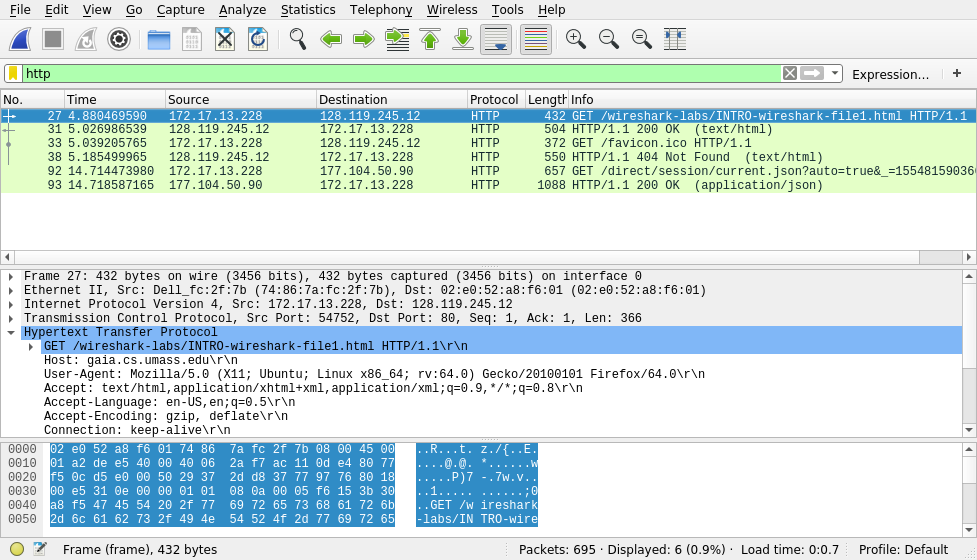
\includegraphics[width=\linewidth]{part-01/ex-1-1-1.png}
      \captionof{figure}{Versão HTTP utilizada.}
      \label{fig:p1-1-1-1}
      \vspace{1em}

      Tanto o navegador quanto o servidor web utilizam HTTP 1.1.
    \end{solution}

    \pagebreak
    \subpart
    Línguas que o navegador aceita.

    \begin{solution}
      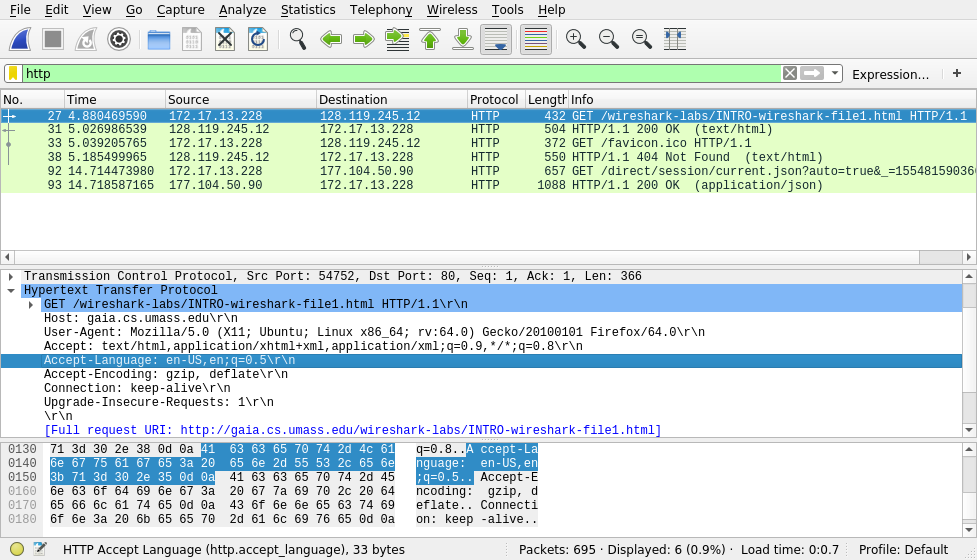
\includegraphics[width=\linewidth]{part-01/ex-1-1-2.png}
      \captionof{figure}{Línguas aceitas pelo Firefox.}
      \vspace{1em}

      O navegador aceita como língua apenas inglês dos EUA.
    \end{solution}

    \subpart
    IP do seu computador e do servidor.

    \begin{solution}
      O computador possui IP \verb|172.17.13.228| e o servidor
      \verb|128.119.245.12|, como pode-se observar nas colunas
      \emph{Source} e \emph{Destination} da linha selecionada
      na Figura \ref{fig:p1-1-1-1}, respectivamente.      
    \end{solution}

    \subpart
    Código de \emph{status} retornado do servidor para o navegador.

    \begin{solution}
      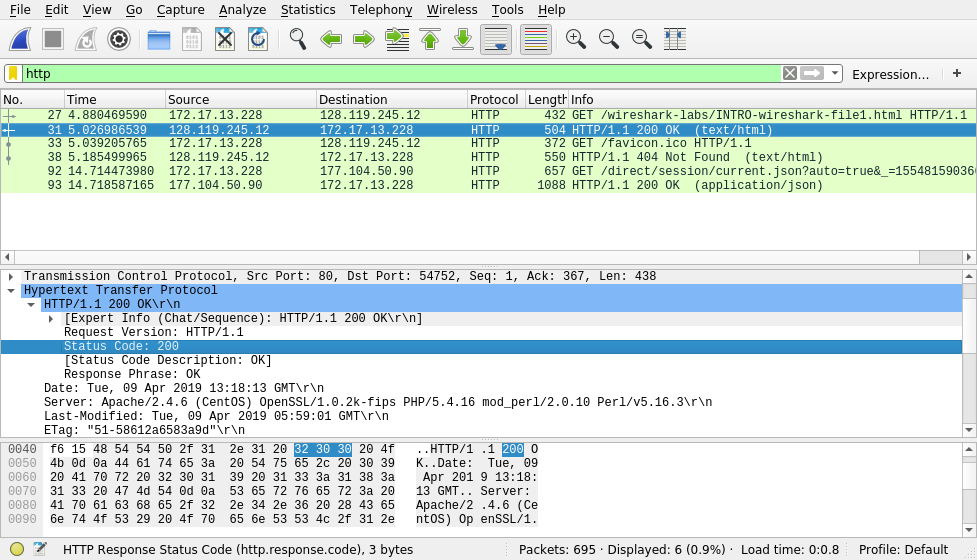
\includegraphics[width=\linewidth]{part-01/ex-1-1-4.png}
      \captionof{figure}{Código de resposta}
      \vspace{1em}

      O servidor retorna um status \verb|200|, sinalizando que a
      requisição foi aceita sem problemas. O \emph{status}
      serve para identificar o tipo da resposta dada para o
      cliente.   
    \end{solution}

    \subpart
    HTTP persistente ou não persistente.

    \begin{solution}
      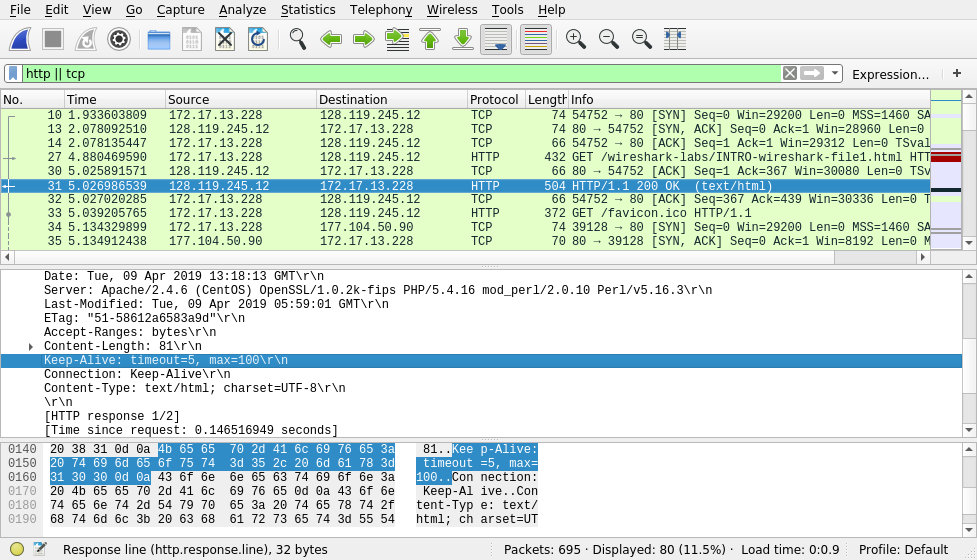
\includegraphics[width=\linewidth]{part-01/ex-1-1-5.png}
      \captionof{figure}{Persistência.}
      \vspace{1em}

      É uma conexão HTTP persistente. Antes de efetuar o
      \verb|GET|, estabelece-se uma conexão TCP. O parâmetro
      \emph{keep-alive} no cabeçalho da resposta faz com que
      esta conexão fique viva durante \SI{5}{\second}, assim,
      após o \emph{download} ser concluído, esta é encerrada.
    \end{solution}

    \subpart
    Última modificação do arquivo HTML do servidor.

    \begin{solution}
      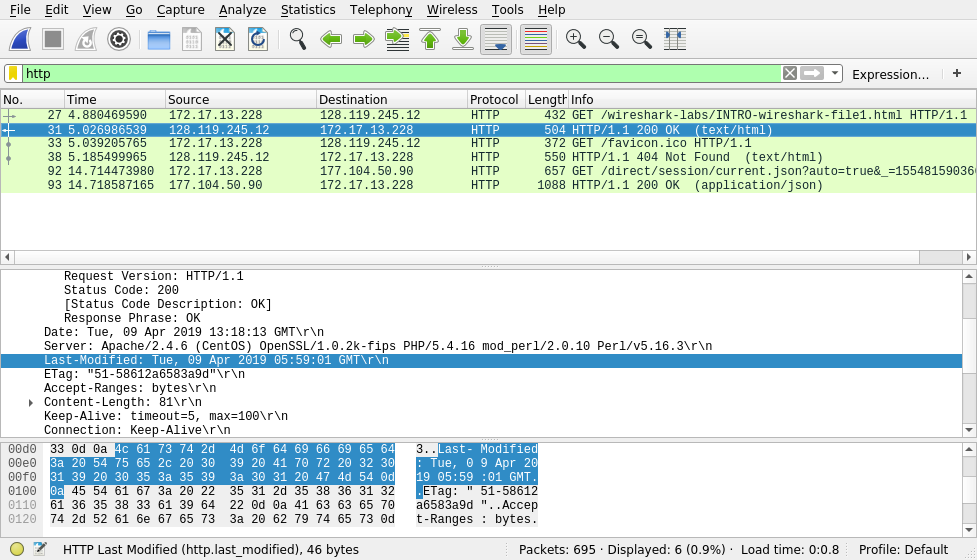
\includegraphics[width=\linewidth]{part-01/ex-1-1-6.png}
      \captionof{figure}{Data da última modificação.}
      \vspace{1em}

      A última modificação do arquivo ocorreu em 09 de Abril.
      Esta informação é utilizada para o \emph{cache} da máquina.
    \end{solution}

    \pagebreak
    \subpart
    Número de \emph{bytes} de conteúdo retornado ao navegador.

    \begin{solution}
      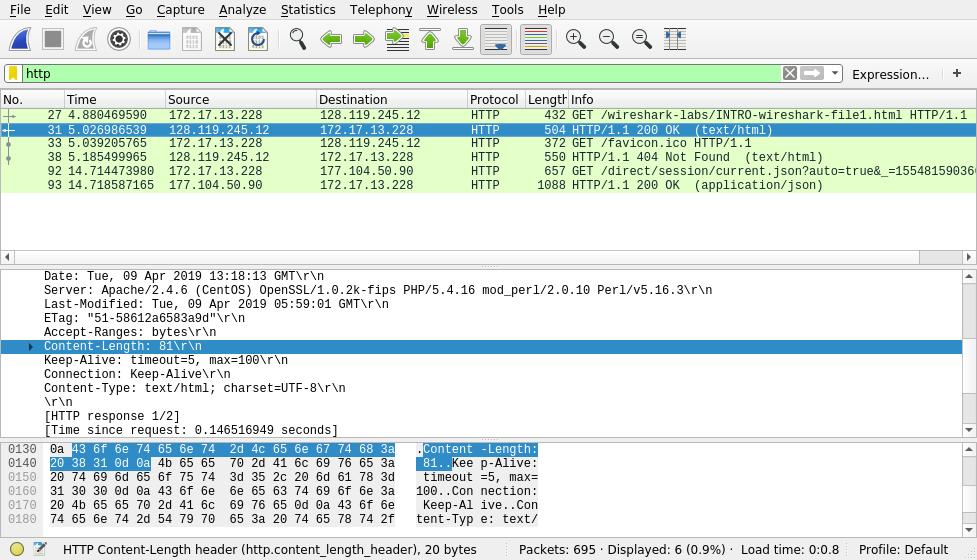
\includegraphics[width=\linewidth]{part-01/ex-1-1-7.png}
      \captionof{figure}{Tamanho da resposta.}
      \vspace{1em}

      O conteúdo enviado ao navegador possui \SI{81}{bytes}.
    \end{solution}
  \end{subparts}

  \part
  Analise os dados (\emph{raw data}) do pacote e desecreva o
  que é possível observar.

  \begin{solution}
    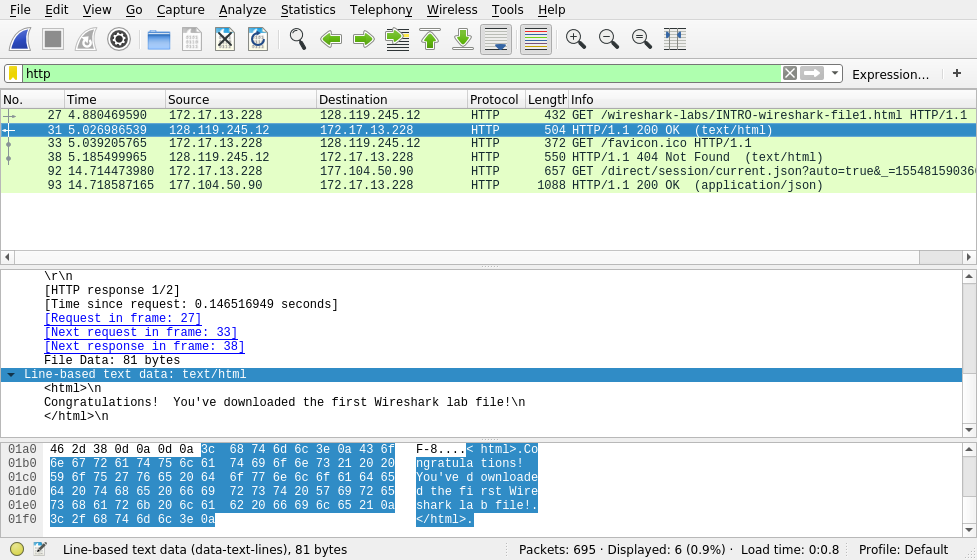
\includegraphics[width=\linewidth]{part-01/ex-1-2.png}
    \captionof{figure}{Conteúdo da resposta.}
    \vspace{1em}

    Pode-se observar a resposta, que é o código HTML retornado
    ao navegador, na qual o renderizará corretamente após
    o \emph{download}.
  \end{solution}
\end{parts}

\question
\verb|GET| condicional.

\begin{parts}
  \part
  Limpe o \emph{cache} do seu navegador e acesse a página
  \url{http://gaia.cs.umass.edu/wireshark-labs/HTTP-wireshark-file2.html}.

  \part
  Verifique o conteúdo da primeira requisição \verb|GET|. É possível
  ver \verb|IF-MODIFIED-SINCE| no HTTP \verb|GET|?

  \begin{solution}
    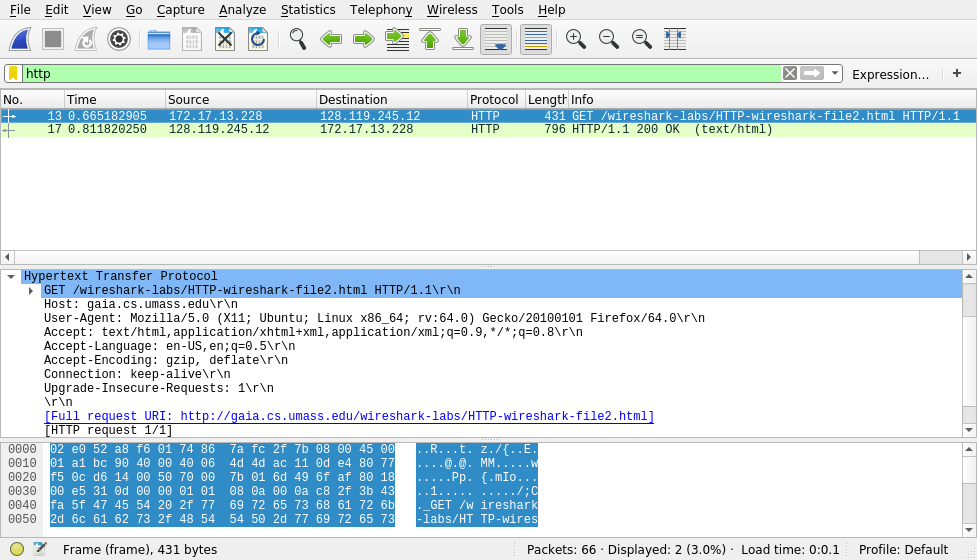
\includegraphics[width=\linewidth]{part-01/ex-2-2.png}
    \captionof{figure}{Cabeçalho da requisição.}
    \vspace{1em}

    Não há a presença de \verb|IF-MODIFIED-SINCE| no \verb|GET|
    pois é a primeira vez que se acessa esta página nesta máquina,
    visto que o \emph{cache} foi limpado.
  \end{solution}

  \part
  Verifique a resposta do servidor. O servidor retorna o conteúdo
  do arquivo?

  \begin{solution}
    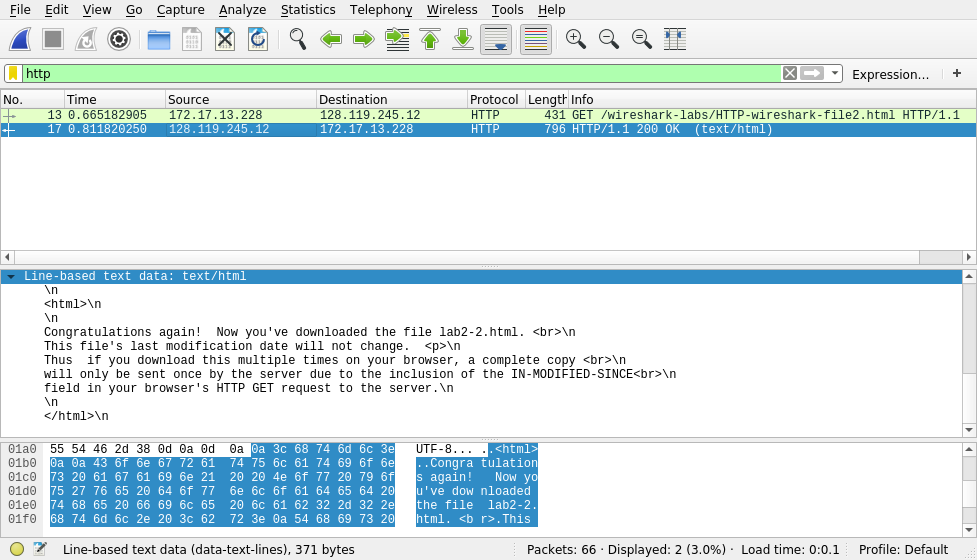
\includegraphics[width=\linewidth]{part-01/ex-2-3.png}
    \captionof{figure}{Conteúdo do arquivo.}
    \vspace{1em}

    O servidor retorna o conteúdo do arquivo normalmente, visto
    que é a primeira requisição efetuada da máquina.
  \end{solution}
  
  \part
  Faça uma segunda requisição \verb|GET| e verifique a resposta
  do servidor. É possível ver\\ \verb|IF-MODIFIED-SINCE| no HTTP
  \verb|GET|? Explique.

  \begin{solution}
    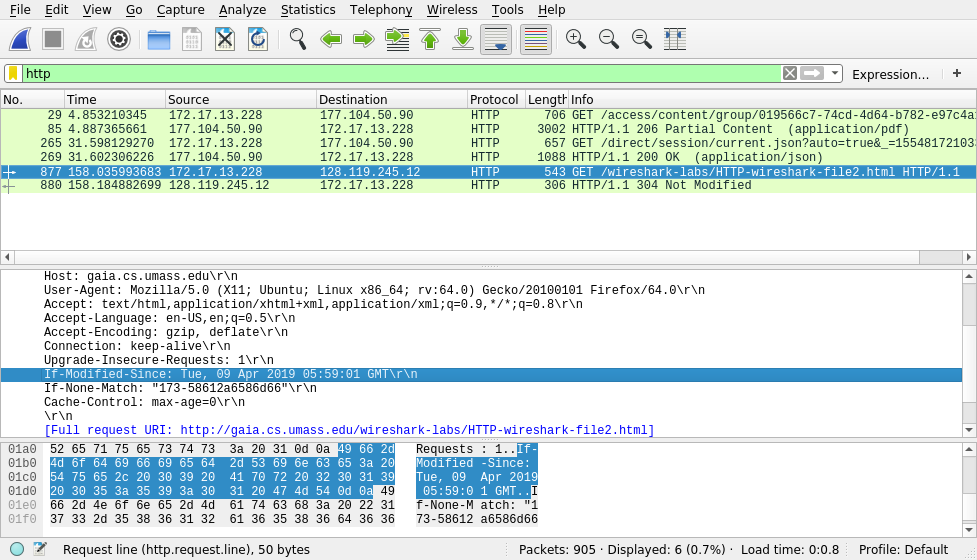
\includegraphics[width=\linewidth]{part-01/ex-2-4.png}
    \captionof{figure}{Presença do campo no \texttt{GET}.}
    \vspace{1em}

    Sim, é possível ver o campo no \verb|GET|, já que utiliza-se
    para a máquina utilizar seu próprio \emph{cache} caso
    a página não tenha sido modificada no servidor.
  \end{solution}

  \part
  Verifique a resposta do servidor ao segundo \verb|GET|.
  O servidor retorna o conteúdo do arquivo? Explique.

  \begin{solution}
    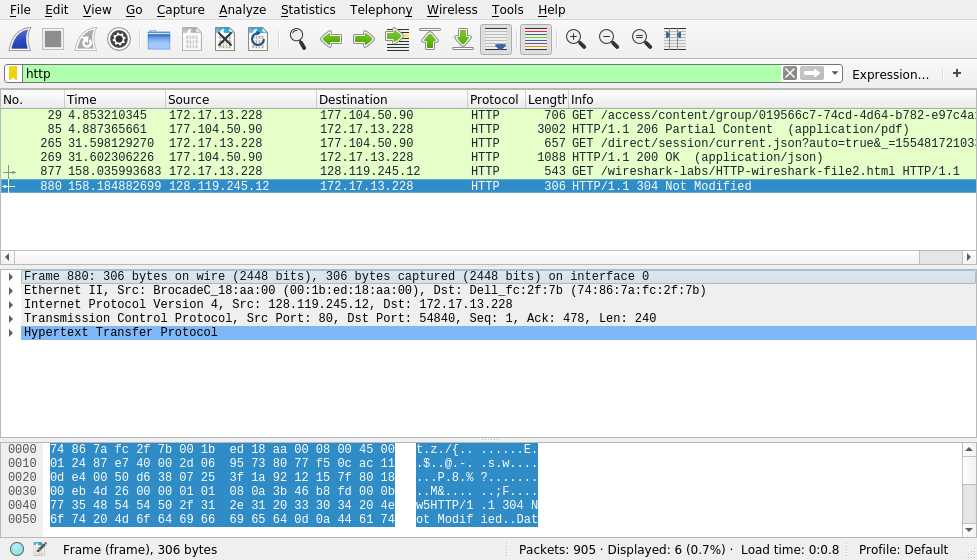
\includegraphics[width=\linewidth]{part-01/ex-2-5.png}
    \captionof{figure}{Resposta não enviada.}
    \vspace{1em}

    A resposta não é enviada, no lugar retorna-se um \emph{status}
    \verb|304|, que sinaliza que o conteúdo no servidor não
    foi modificado, portanto a máquina pode utilizar o seu \emph{cache}.
  \end{solution}
\end{parts}

\question
HTML com objetos.

\begin{parts}
  \part
  Acesse a página \url{http://gaia.cs.umass.edu/wireshark-labs/HTTP-wireshark-file4.html}.

  \part
  Quantas requisições HTTP \verb|GET| foram feitas pelo navegador?
  Para qual endereço IP estas requisições foram feitas?

  \begin{solution}
    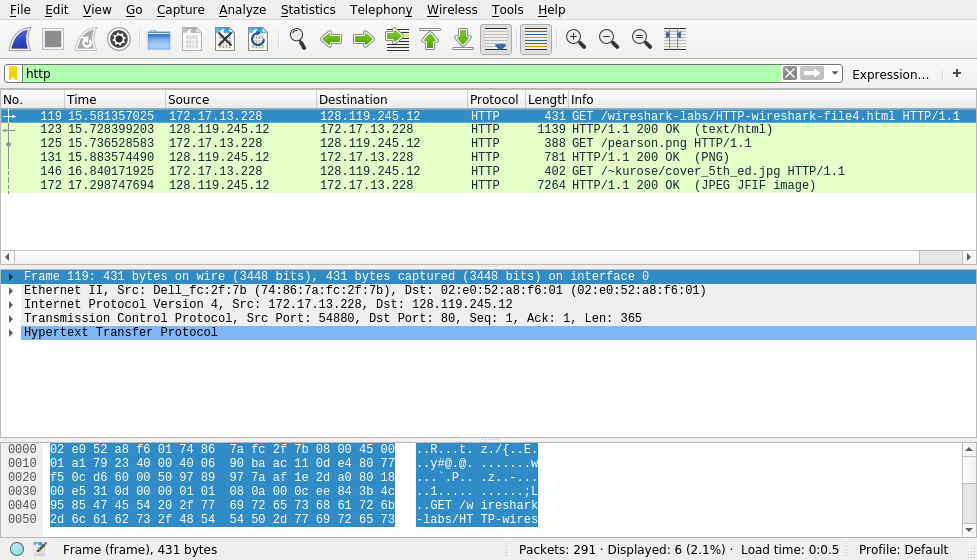
\includegraphics[width=\linewidth]{part-01/ex-3-2.png}
    \captionof{figure}{Requisições efetuadas.}
    \vspace{1em}

    Foram realizadas três requisições. Quando o navegador recebe o HTML,
    verifica-se que há a presença de duas imagens, então o mesmo realiza
    uma requisição para cada uma, totalizando portanto três requisições
    ao todo.
  \end{solution}

  \part
  Identifique se o navegador fez o \emph{download} das imagens (objetos)
  de maneira serial ou paralela. Explique.

  \begin{solution}
    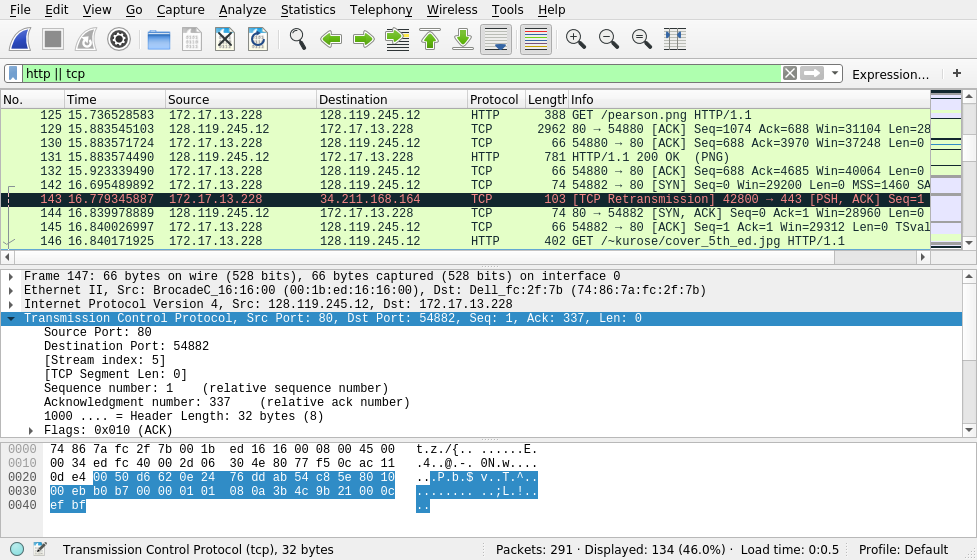
\includegraphics[width=\linewidth]{part-01/ex-3-3.png}
    \captionof{figure}{Terceira requisição.}
    \vspace{1em}

    O navegador fez o \emph{download} das imagens paralelamente. A primeira
    conexão TCP foi estabelecida na porta \verb|54480| e a segunda na
    \verb|54482|, onde há uma \emph{thread} para cada uma.
  \end{solution}
\end{parts}

\question
Autenticação HTTP.

\begin{parts}
  \part
  \sloppy
  Acesse a página \url{http://gaia.cs.umass.edu/wireshark-labs/protected_pages/HTTP-wireshark-file5.html}
  com nome de usuário \verb|wireshark-students| e senha \verb|network|.

  \part
  Qual a resposta do servidor ao HTTP \verb|GET| inicial do navegador?

  \begin{solution}
    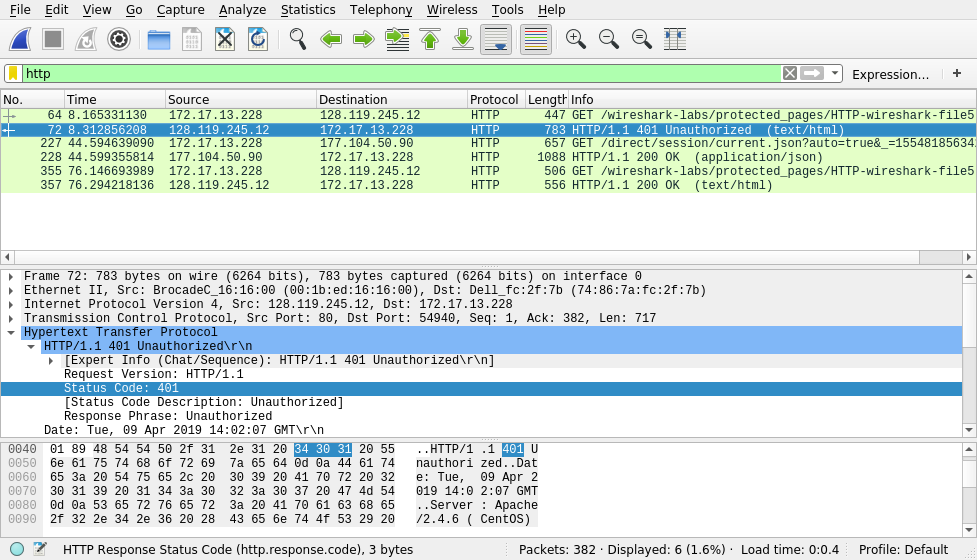
\includegraphics[width=\linewidth]{part-01/ex-4-2.png}
    \captionof{figure}{Resposta inicial.}
    \vspace{1em}

    A resposta do servidor ao \verb|GET| realizado inicialmente do
    navegador foi \verb|401|, que sinaliza ao navegador que o mesmo
    não está autorizado a requisitar tal endereço, informando-o
    que deve informar um usuário e senha.
  \end{solution}

  \part
  Na segunda mensagem \verb|GET| do navegador, qual novo campo é incluído
  na mensagem \verb|GET|?

  \begin{solution}
    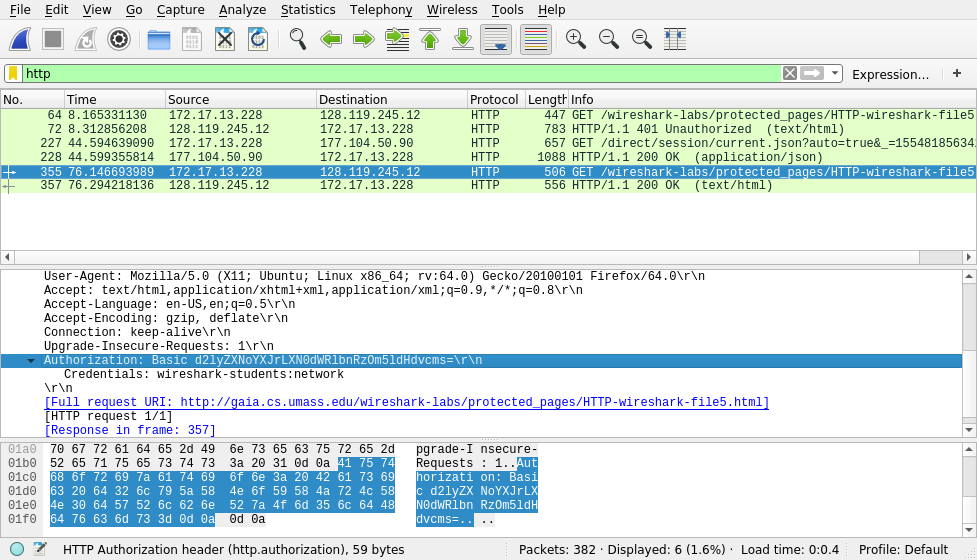
\includegraphics[width=\linewidth]{part-01/ex-4-3.png}
    \captionof{figure}{Campo novo incluido.}
    \label{fig:p1-4-3}
    \vspace{1em}

    O navegador inclui no cabeçalho da requisição o campo \verb|Authorization|,
    que inclui o método de autenticação utilizado.
  \end{solution}

  \part
  É possível visualizar o nome de usuário e senha no pacote capturado
  pelo wireshark? Discuta sobre a segurança desta autenticação HTTP.

  \begin{solution}
    Sim, é possível visualizar o nome de usuário e senha no pacote capturado,
    como pode-se observar na Figura \ref{fig:p1-4-3}. Tal fato se deve
    pelo funcionamento desta autenticação. O usuário e senha são encodados
    em base 64 e enviados diretamente, permitindo qualquer tipo de interceptação,
    visto que não se utiliza um protocolo mais seguro como o HTTPS, recomendado
    pelo navegador.
  \end{solution}
\end{parts}

\question
Resolução de nomes.

\begin{parts}
  \part
  Acesse o site \url{www.ipv6.br} e filtre as mensagens DNS.

  \part
  O protocolo DNS usa TCP ou UDP?

  \begin{solution}
    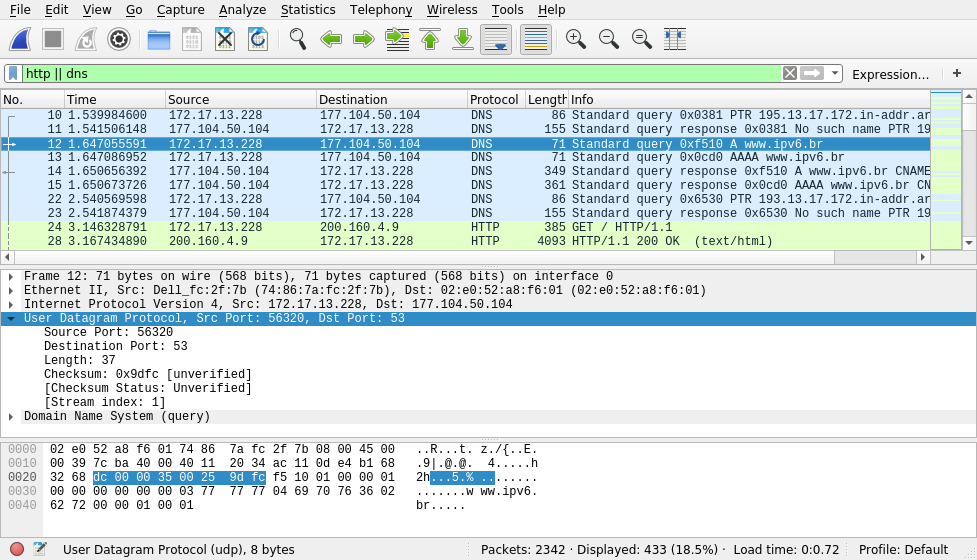
\includegraphics[width=\linewidth]{part-01/ex-5-2.png}
    \captionof{figure}{Protocolo UDP dentro do DNS.}
    \label{fig:p1-5-2}
    \vspace{1em}

    O protocolo utiliza UDP já que não há a necessidade de conexão, visto
    que a quantidade de perguntas não altera a resposta, além de possibilitar
    com que se possa perguntar a mais de um servidor.
  \end{solution}

  \part
  Identifique a porta de destino da mensagem \verb|query| DNS e a porta
  de origem da mensagem de resposta do DNS.

  \begin{solution}
    Como pode-se observar na Figura \ref{fig:p1-5-2}, a porta de destino
    do \emph{query} DNS é a \verb|53|, a porta padrão. A porta de origem
    da resposta do DNS também é a \verb|53|.
  \end{solution}

  \part
  Identifique o endereço IP para qual a mensagem de \verb|query| do DNS
  foi enviada.

  \begin{solution}
    Como também pode-se observar na Figura \ref{fig:p1-5-2}, na coluna
    \emph{Destination} do pacote selecionado, a mensagem de \emph{query}
    do DNS foi enviada ao endereço IP \verb|177.10.50.104|, que é o
    DNS padrão da UFABC, o \verb|ns4.ufabc.edu.br|.
  \end{solution}

  \part
  Examine a resposta DNS. Quantas ``respostas'' foram dadas? Qual o 
  conteúdo destas respostas?

  \begin{solution}
    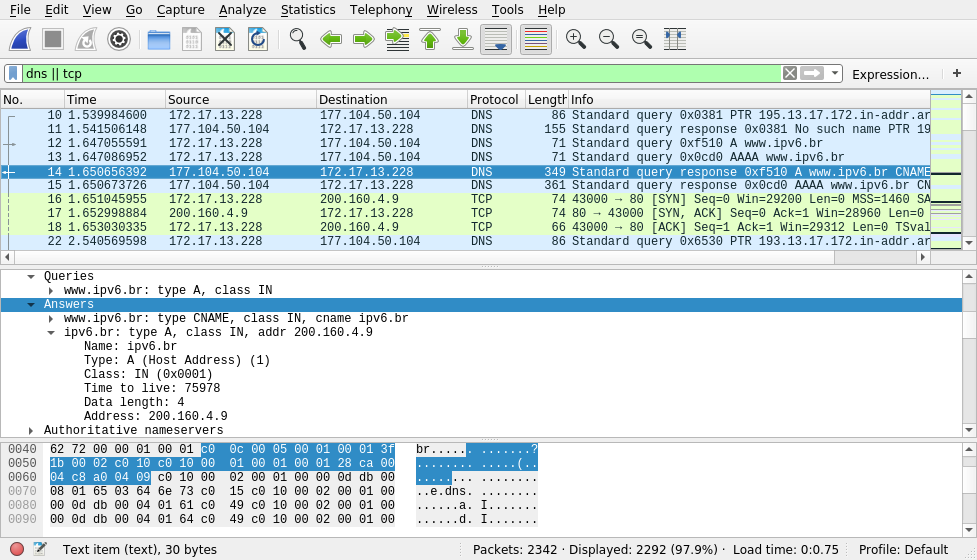
\includegraphics[width=\linewidth]{part-01/ex-5-5.png}
    \captionof{figure}{Respostas enviadas pelo DNS.}
    \vspace{1em}

    São dadas duas respostas. O conteúdo informa o nome requisitado,
    bem como seu tipo (\verb|A (Host Address)|) e o endereço
    resolvido, neste caso sendo \verb|200.160.4.9|, sendo
    um endereço IPv4.
  \end{solution}

  \part
  Aplique os filtros necessários e considere o pacote TCP SYN subsequente
  enviado pelo navegador. O IP de destino do pacote TCP SYN corresponde
  ao endereço IP fornecido pela mensagem de resposta DNS?

  \begin{solution}
    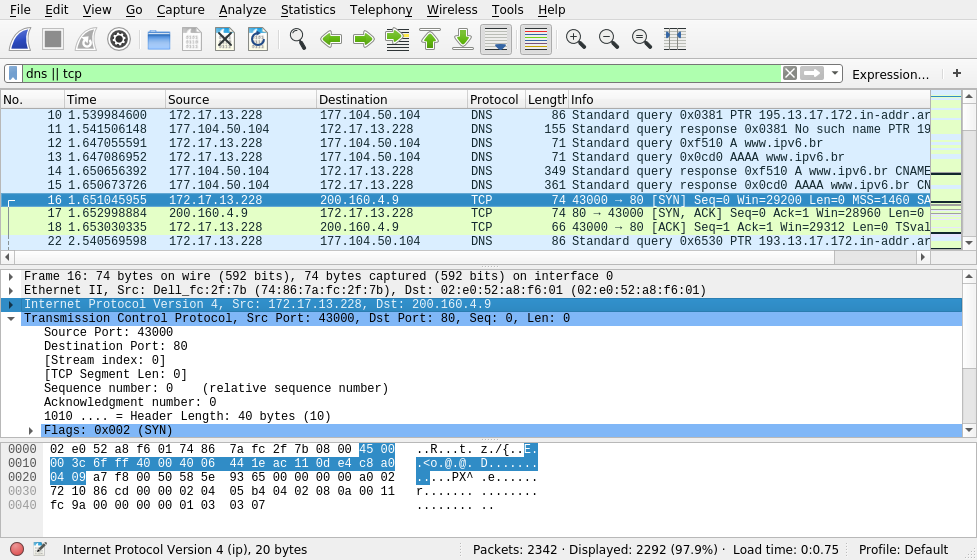
\includegraphics[width=\linewidth]{part-01/ex-5-6.png}
    \captionof{figure}{Pacote TCP subsequente.}
    \vspace{1em}

    Sim, o IP de destino do pacote TCP SYN é o mesmo endereço fornecido
    pela mensagem de resposta de DNS. Tal fato se comprova pelo funcionamento
    do método, o DNS resolve o nome e o TCP inicia a conexão com o IP recebido.
  \end{solution}

  \part
  Esta página contém imagens. Antes de requisitar cada imagem, seu
  \emph{host} faz novas \emph{queries} DNS?

  \begin{solution}
    Não, o \emph{host} não faz novas \emph{queries} DNS visto que como as
    imagens estão localizadas no mesmo servidor, utiliza-se o \emph{cache}
    diretamente para obter o IP, não necessitando realizar novos \emph{queries}
    para o servidor DNS em relação ao mesmo nome.
  \end{solution}
\end{parts}

\question
Usando \verb|nslookup|.

\begin{parts}
  \part
  Execute o comando \verb|nslookup www.mit.edu|.

  \begin{solution}
    O comando foi executado corretamente.

    \begin{Verbatim}[label={\$ nslookup www.mit.edu}]
    Server:         127.0.1.1
    Address:        127.0.1.1#53

    Non-authoritative answer:
    www.mit.edu     canonical name = www.mit.edu.edgekey.net.
    www.mit.edu.edgekey.net canonical name = e9566.dscb.akamaiedge.net.
    Name:   e9566.dscb.akamaiedge.net
    Address: 23.38.154.77
    \end{Verbatim}
  \end{solution}

  \part
  Identifique a porta de destino da mensagem de \emph{query} DNS e a porta
  de origem da mensagem de resposta do DNS.

  \begin{solution}
    Utiliza-se novamente a mesma porta de destino e de origem, a porta
    \verb|53|, que é o esperado para o Linux. No caso do Windows, a porta 
    pode variar.
  \end{solution}

  \part
  Identifique o endereço IP para qual a mensagem de \emph{query} DNS
  foi enviada.

  \begin{solution}
    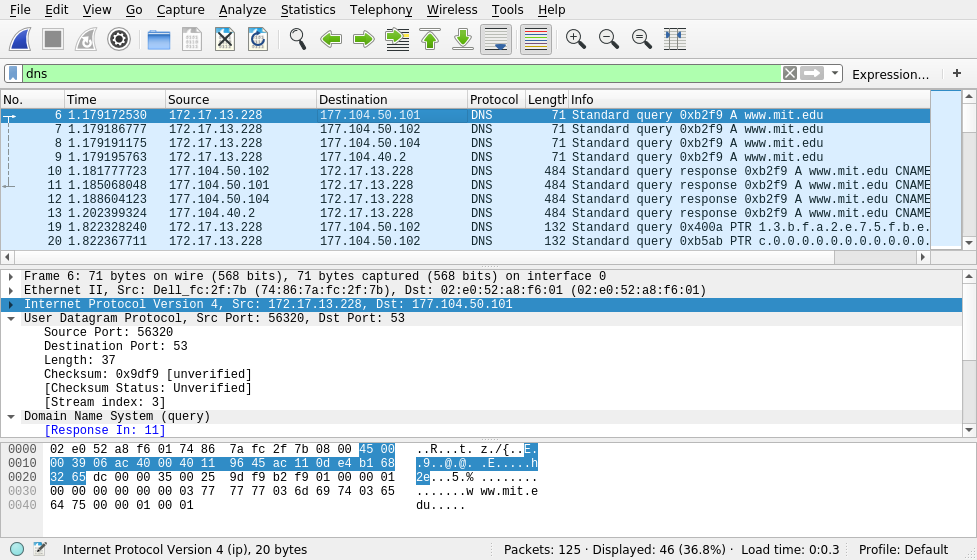
\includegraphics[width=\linewidth]{part-01/ex-6-3.png}
    \captionof{figure}{Mensagens enviadas.}
    \vspace{1em}

    A mensagem de \emph{query} DNS foi enviada para os servidores de DNS
    da UFABC, os quais podem ser observados na figura acima: 
    
    \begin{itemize}
      \item \verb|ns4.ufabc.edu.br (177.10.50.104)|
      \item \verb|ns3.ufabc.edu.br (177.104.40.2)|
      \item \verb|ns2.ufabc.edu.br (177.104.50.102)|
      \item \verb|ns1.ufabc.edu.br (177.104.50.101)|
    \end{itemize}
  \end{solution}

  \part
  Examine a resposta DNS. Quantas ``respostas'' foram dadas? Qual
  o conteúdo destas respostas?

  \begin{solution}
    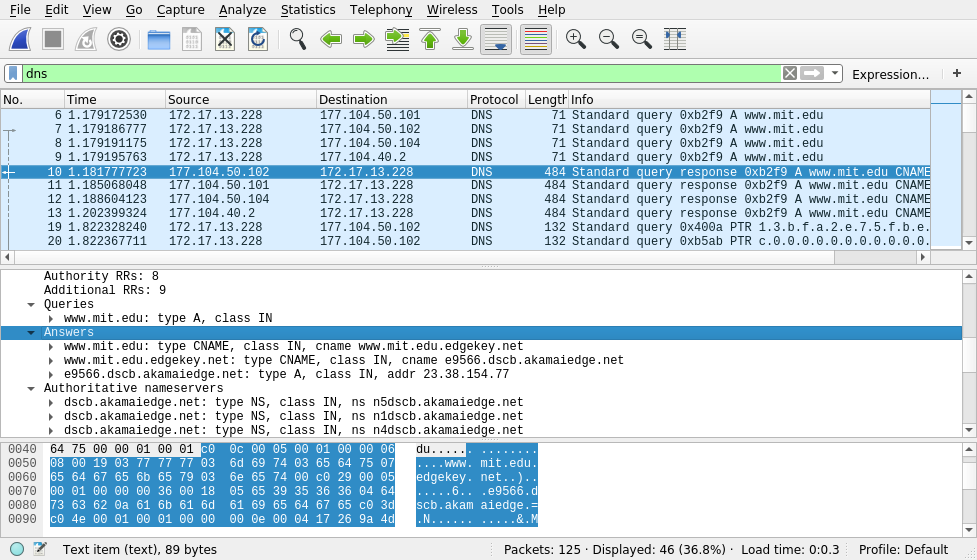
\includegraphics[width=\linewidth]{part-01/ex-6-4.png}
    \captionof{figure}{Respostas recebidas.}
    \vspace{1em}

    Foram recebidas quatro respostas, uma de cada servidor de DNS
    as quais as \emph{queries} foram enviadas, listados no exercício
    anterior. Todas as respostas possuem as mesmas resoluções
    de endereço IP mostradas na figura acima.
  \end{solution}

  \part
  Execute o comando \verb|nslookup www.aiit.or.kr google-public-dns-a.google.com|.

  \begin{solution}
    O comando foi executado corretamente.

    \begin{Verbatim}[label={\$ nslookup www.aiit.or.kr google-public-dns-a.google.com}]
    Server:         google-public-dns-a.google.com
    Address:        8.8.8.8#53

    Non-authoritative answer:
    Name:   www.aiit.or.kr
    Address: 58.229.6.225
    \end{Verbatim}
  \end{solution}

  \part
  Identifique o endereço IP para qual a mensagem de \emph{query} do DNS
  foi enviada. Este endereço IP é o mesmo do seu servidor DNS local?
  Caso contrário, esse endereço IP corresponde a que servidor?

  \begin{solution}
    A mensagem de \emph{query} do DNS foi enviada ao endereço IP
    \verb|8.8.8.8|, que não é o mesmo do servidor de DNS local,
    correspondendo ao endereço do Serviço de DNS Público do Google.
  \end{solution}

  \part
  Examine a resposta DNS. Quantas ``respostas'' foram dadas? Qual o
  conteúdo destas respostas?

  \begin{solution}
    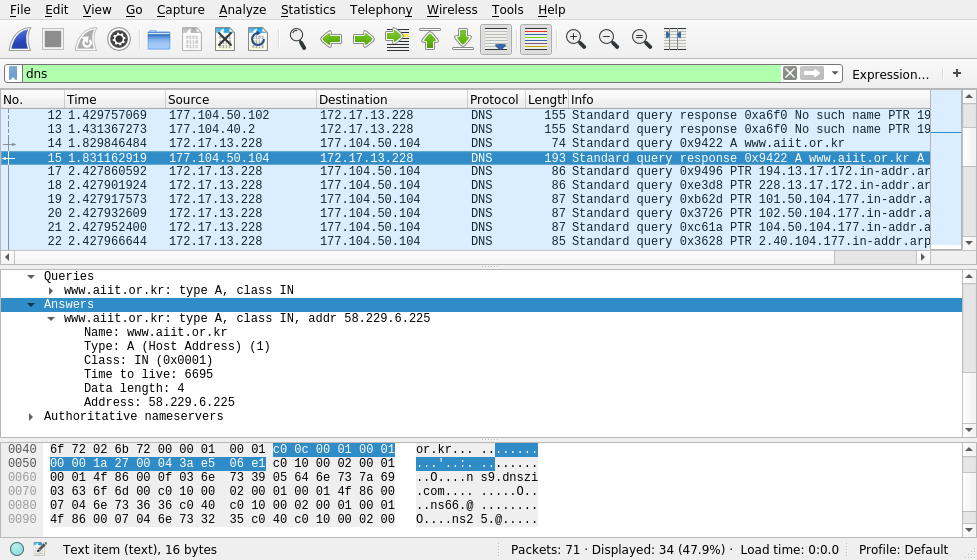
\includegraphics[width=\linewidth]{part-01/ex-6-7.png}
    \captionof{figure}{Resposta recebida.}
    \vspace{1em}

    Foram recebidas uma resposta, já que se especifica que se utilizará
    apenas o servidor do Google. No caso, o nome foi resolvido para
    o endereço IP \verb|58.229.6.225|.
  \end{solution}
\end{parts}

  \end{questions}
  \pagebreak
  \begin{questions}
    \section*{Parte 02}
    \question
Aplicação cliente-servidor TCP.

\begin{parts}
  \part
  Execute primeiro o servidor (\verb|TCPServer.java|) e depois o
  cliente (\verb|TCPClient.java|). O que aconteceu?

  \begin{solution}
    O servidor estabelece um \verb|ServerSocket|, ficando em um loop 
    infinito esperando por uma conexão. Se houver uma conexão, o servidor
    lê as \verb|Strings| enviadas pelo cliente, passando-as para maiúscula
    e devolvendo para o mesmo. A abstração utilizada no \emph{socket}
    é uma de fluxo, onde há um de entrada, pelo teclado, e saída,
    para envio dos dados. A conexão entre servidor-cliente é mantida
    até que o cliente envie uma linha em branco.

    \begin{Verbatim}[label={\$ java TCPServer}]
    Waiting for connection at port 9000.
    Connection established from /127.0.0.1
    Waiting for connection at port 9000.
    \end{Verbatim}

    \begin{Verbatim}[label={\$ java TCPClient}]
    Ola, este eh um teste
    OLA, ESTE EH UM TESTE
    Mensagem para o servidor
    MENSAGEM PARA O SERVIDOR
   
    \end{Verbatim}
  \end{solution}

  \part
  Execute primeiro o cliente e depois o servidor. O que aconteceu?
  Justifique.

  \begin{solution}
    Para o cliente estabelecer uma conexão com o servidor, este deve
    já estar operando. Caso o servidor não esteja operando, a camada
    de transporte do servidor enviará uma mensagem ao cliente informando
    que não é possível estabelecer uma conexão, gerando uma exceção no
    Java, onde a conexão é recusada.

    \begin{Verbatim}[label={\$ java TCPClient}, fontsize=\scriptsize]
    Exception in thread "main" java.net.ConnectException: Conexão recusada (Connection refused)
      at java.net.PlainSocketImpl.socketConnect(Native Method)
      at java.net.AbstractPlainSocketImpl.doConnect(AbstractPlainSocketImpl.java:350)
      at java.net.AbstractPlainSocketImpl.connectToAddress(AbstractPlainSocketImpl.java:206)
      at java.net.AbstractPlainSocketImpl.connect(AbstractPlainSocketImpl.java:188)
      at java.net.SocksSocketImpl.connect(SocksSocketImpl.java:392)
      at java.net.Socket.connect(Socket.java:589)
      at java.net.Socket.connect(Socket.java:538)
      at java.net.Socket.<init>(Socket.java:434)
      at java.net.Socket.<init>(Socket.java:211)
      at TCPClient.main(TCPClient.java:11)
    \end{Verbatim}

    \begin{Verbatim}[label={\$ java TCPServer}]
    Waiting for connection at port 9000.    
    \end{Verbatim}
  \end{solution}

  \part
  Altere as portas do servidor e cliente. O que acontece se as portas
  forem diferentes? Justifique.

  \begin{solution}
    Para se estabelecer uma comunicação, além do número do IP
    é necessário saber a qual processo ela se direciona. Logo,
    como o servidor opera na porta \verb|9000|, o cliente precisa 
    necessariamente utilizar esta porta para estabelecer uma conexão
    e trocar os dados sem nenhum problema.

    \begin{Verbatim}[label={\$ java TCPServer}]
    Waiting for connection at port 9000.
    \end{Verbatim}

    \begin{Verbatim}[label={\$ java TCPClient}, fontsize=\scriptsize]
    Exception in thread "main" java.net.ConnectException: Conexão recusada (Connection refused)
      at java.net.PlainSocketImpl.socketConnect(Native Method)
      at java.net.AbstractPlainSocketImpl.doConnect(AbstractPlainSocketImpl.java:350)
      at java.net.AbstractPlainSocketImpl.connectToAddress(AbstractPlainSocketImpl.java:206)
      at java.net.AbstractPlainSocketImpl.connect(AbstractPlainSocketImpl.java:188)
      at java.net.SocksSocketImpl.connect(SocksSocketImpl.java:392)
      at java.net.Socket.connect(Socket.java:589)
      at java.net.Socket.connect(Socket.java:538)
      at java.net.Socket.<init>(Socket.java:434)
      at java.net.Socket.<init>(Socket.java:211)
      at TCPClient.main(TCPClient.java:11)
    \end{Verbatim}
  \end{solution}

  \part
  Execute servidor e cliente em máquinas diferentes. Em seguida, envie
  várias mensagens ao servidor a partir de várias máquinas diferentes
  (ao mesmo tempo!). O que aconteceu? Justifique.

  \begin{solution}
    Não é possível estabelecer uma conexão com o servidor quando
    um cliente já está conectado ao servidor, já que a comunicação
    é sempre um-para-um, uma relação entre o \emph{host} de origem e o
    \emph{host} de destino. Para permitir que múltiplos clientes
    se conectem ao servidor, será necessário modificar seu código.

    \begin{Verbatim}[label={\$ java TCPServer}]
    Waiting for connection at port 9000.
    Connection established from /172.17.13.228
    Waiting for connection at port 9000
    \end{Verbatim}

    \begin{Verbatim}[label={\$ java TCPClient}]
    Este eh um teste
    ESTE EH UM TESTE
    Enviando de maquina diferente
    ENVIANDO DE MAQUINA DIFERENTE

    \end{Verbatim}
  \end{solution}

  \part
  Verifique o cliente e servidor UDP da aula anterior. Quais as
  principais diferenças para o cliente e servidor TCP?

  \begin{solution}
    No UDP não se estabelece uma conexão entre cliente-servidor.
    O servidor recebe os datagramas e envia esses datagramas.
    Já no TCP é necessário estabelecer uma conexão para a comunicação,
    além do fato que o servidor somente aceita um cliente conectado
    por vez. No UDP também não é necessário encerrar a conexão,
    visto que ela nunca é estabelecida, enquanto no TCP é necessário
    encerrar a conexão para liberar o servidor.
  \end{solution}

  \part
  Modifique o programa cliente para que permaneça conectado enviando
  mensagens ao servidor. A conexão só será desfeita se o cliente enviar
  o comando ``tchau'' para o servidor. Faça também as modificações
  necessárias no código do servidor.

  \begin{solution}
    Modificou-se a verificação no cliente para quando o usuário dava
    um enter para sinalizar que queria encerrar a conexão. Após o usuário
    enviar o comando ``tchau'', este comando é enviado ao servidor e o
    cliente se desconecta, bem como o servidor que identifica o comando
    e se desconecta também.\\

    \begin{Verbatim}[label={\$ java TCPServerModified}]
    Waiting for connection at port 9000.
    Connection established from /127.0.0.1
    Waiting for connection at port 9000.
    \end{Verbatim}

    \begin{Verbatim}[label={\$ java TCPClientModified}]
    Ola, este eh um teste
    OLA, ESTE EH UM TESTE
    Tambem um teste
    TAMBEM UM TESTE
    tchau
    \end{Verbatim}
  \end{solution}
\end{parts}

\question
Desenvolvimento de um servidor TCP com múltiplos clientes.

\begin{parts}
  \part
  Implemente um servidor que atenda a vários clientes simultaneamente.

  \begin{solution}
    O servidor fica em um \emph{loop} infinito aguardando por conexões,
    quando ele recebe alguma, inicia-se uma nova \emph{thread} para
    a conexão, permitindo com que vários clientes sejam atendidos
    ao mesmo tempo.

    \begin{Verbatim}[label={\$ java TCPServerMultiple}]
    Waiting for connection at port 9000.
    Waiting for connection at port 9000.
    Connection established from /172.17.13.228
    Waiting for connection at port 9000.
    Connection established from /172.17.13.220
    \end{Verbatim}

    \begin{Verbatim}[label={\$ java TCPClient [172.17.13.220]}]
    Este eh um teste
    ESTE EH UM TESTE
    Tambem um teste
    TAMBEM UM TESTE

    \end{Verbatim}

    \begin{Verbatim}[label={\$ java TCPClient [172.17.13.228]}]
    Enviando da outra maquina
    ENVIANDO DA OUTRA MAQUINA
    Por enquanto tah tudo tranquilo
    POR ENQUANTO TAH TUDO TRANQUILO

    \end{Verbatim}
  \end{solution}
\end{parts}

  \end{questions}
\end{document}
